% This file was created by matlab2tikz.
%
%The latest updates can be retrieved from
%  http://www.mathworks.com/matlabcentral/fileexchange/22022-matlab2tikz-matlab2tikz
%where you can also make suggestions and rate matlab2tikz.
%
\definecolor{mycolor1}{rgb}{0.00000,0.44700,0.74100}%
%
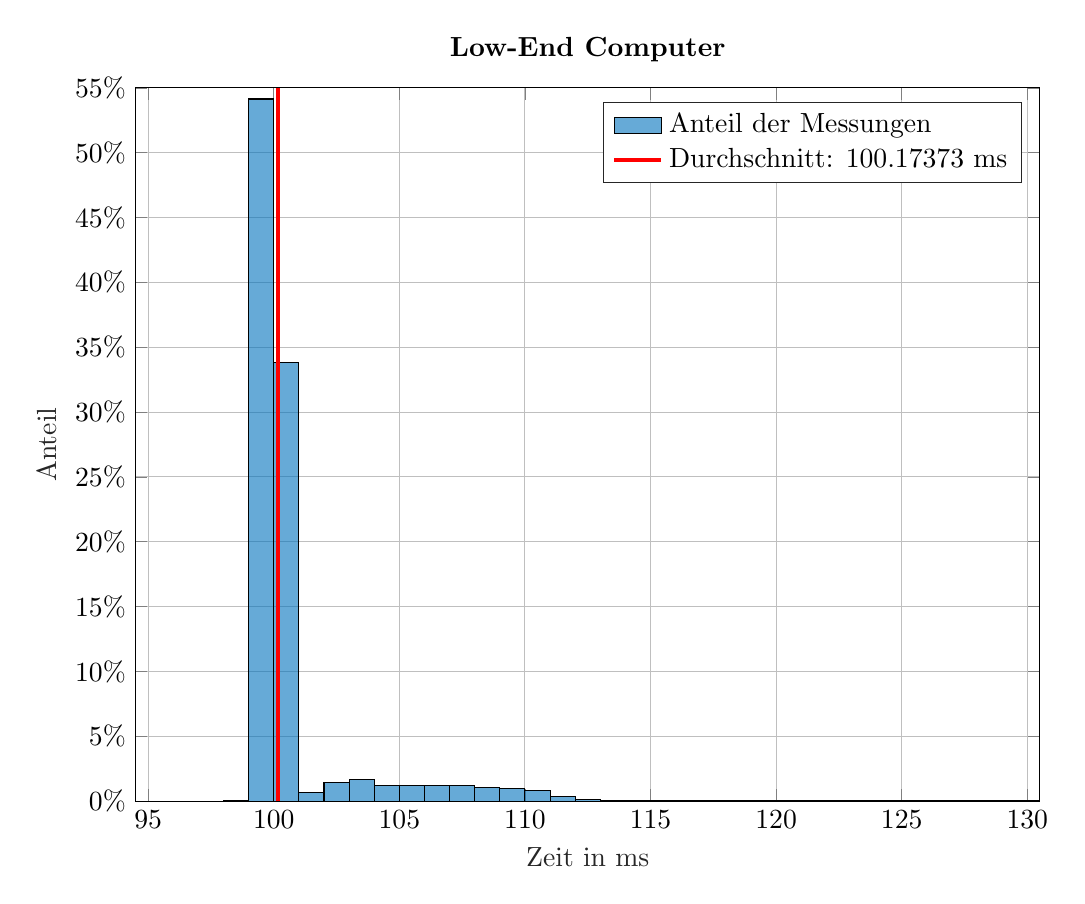
\begin{tikzpicture}

\begin{axis}[%
width=4.521in,
height=3.566in,
at={(0.758in,0.481in)},
scale only axis,
xmin=94.5,
xmax=130.5,
xtick={ 95, 100, 105, 110, 115, 120, 125, 130},
xlabel style={font=\color{white!15!black}},
xlabel={Zeit in ms},
ymin=0,
ymax=0.55,
ytick={0,0.05,0.1,0.15,0.2,0.25,0.3,0.35,0.4,0.45,0.5,0.55},
yticklabels={{0\%},{5\%},{10\%},{15\%},{20\%},{25\%},{30\%},{35\%},{40\%},{45\%},{50\%},{55\%}},
ylabel style={font=\color{white!15!black}},
ylabel={Anteil},
axis background/.style={fill=white},
title style={font=\bfseries},
title={Low-End Computer},
xmajorgrids,
ymajorgrids,
legend style={legend cell align=left, align=left, draw=white!15!black}
]
\addplot[ybar interval, fill=mycolor1, fill opacity=0.6, draw=black, area legend] table[row sep=crcr] {%
x	y\\
98	0.0002\\
99	0.54145\\
100	0.338033333333333\\
101	0.0063\\
102	0.0145\\
103	0.0164166666666667\\
104	0.01235\\
105	0.0116666666666667\\
106	0.0119833333333333\\
107	0.0117666666666667\\
108	0.0104666666666667\\
109	0.00998333333333333\\
110	0.0082\\
111	0.00323333333333333\\
112	0.00108333333333333\\
113	0.000266666666666667\\
114	0.000116666666666667\\
115	6.66666666666667e-05\\
116	8.33333333333333e-05\\
117	0.0001\\
118	0.00015\\
119	5e-05\\
120	0.0001\\
121	6.66666666666667e-05\\
122	0.000116666666666667\\
123	0.00015\\
124	0.00015\\
125	0.000166666666666667\\
126	0.00015\\
127	5e-05\\
128	0.0001\\
129	3.33333333333333e-05\\
130	3.33333333333333e-05\\
131	3.33333333333333e-05\\
132	3.33333333333333e-05\\
133	1.66666666666667e-05\\
134	0\\
135	0\\
136	1.66666666666667e-05\\
137	1.66666666666667e-05\\
138	3.33333333333333e-05\\
139	0\\
140	0\\
141	0\\
142	1.66666666666667e-05\\
143	1.66666666666667e-05\\
144	1.66666666666667e-05\\
145	0\\
146	1.66666666666667e-05\\
147	0\\
148	0\\
149	0\\
150	1.66666666666667e-05\\
151	1.66666666666667e-05\\
152	0\\
153	0\\
154	0\\
155	0\\
156	0\\
157	1.66666666666667e-05\\
158	1.66666666666667e-05\\
159	0\\
160	0\\
161	0\\
162	0\\
163	1.66666666666667e-05\\
164	0\\
165	0\\
166	0\\
167	0\\
168	0\\
169	0\\
170	0\\
171	0\\
172	1.66666666666667e-05\\
173	0\\
174	0\\
175	0\\
176	1.66666666666667e-05\\
177	0\\
178	0\\
179	0\\
180	0\\
181	0\\
182	0\\
183	1.66666666666667e-05\\
184	0\\
185	0\\
186	0\\
187	0\\
188	0\\
189	0\\
190	0\\
191	0\\
192	0\\
193	0\\
194	0\\
195	0\\
196	0\\
197	0\\
198	0\\
199	1.66666666666667e-05\\
200	0\\
201	0\\
202	0\\
203	0\\
204	0\\
205	0\\
206	0\\
207	0\\
208	0\\
209	0\\
210	1.66666666666667e-05\\
211	0\\
212	0\\
213	0\\
214	0\\
215	0\\
216	0\\
217	0\\
218	0\\
219	0\\
220	0\\
221	0\\
222	0\\
223	0\\
224	0\\
225	0\\
226	0\\
227	0\\
228	0\\
229	0\\
230	0\\
231	0\\
232	0\\
233	0\\
234	0\\
235	0\\
236	0\\
237	0\\
238	0\\
239	0\\
240	0\\
241	0\\
242	0\\
243	1.66666666666667e-05\\
244	0\\
245	0\\
246	0\\
247	0\\
248	1.66666666666667e-05\\
249	1.66666666666667e-05\\
};
\addlegendentry{Anteil der Messungen}

\addplot [color=red, line width=1.5pt]
  table[row sep=crcr]{%
100.173733333333	0\\
100.173733333333	0.55\\
};
\addlegendentry{Durchschnitt: 100.17373 ms}

\end{axis}
\end{tikzpicture}%